\documentclass{article}
\usepackage{amsmath}
\usepackage{graphicx}
\usepackage{mdframed}
\usepackage[dvipsnames]{xcolor}
\usepackage[colorlinks=true,urlcolor=ForestGreen]{hyperref}
\newcommand{\dspace}{\baselineskip 16pt}
\newcommand{\sspace}{\baselineskip 14pt}
\textheight 9in
\textwidth 6.5in 
\oddsidemargin -0.1in \evensidemargin -0.1in
\topmargin -0.3in
\pagestyle{empty}


\newcounter{problem}[section]
\newenvironment{problem}[1][]{\refstepcounter{problem}\par\medskip
   \noindent \textbf{Problem~\theproblem. #1} \rmfamily}{\medskip}

\newcounter{task}[section]
\newenvironment{task}[1][]{\refstepcounter{task}\par\medskip
   \noindent \textbf{Task~\thetask. #1} \rmfamily}{\medskip}

\newenvironment{proof}{\begin{mdframed}\textbf{Ans:}}{ \end{mdframed}}


\begin{document}
\sspace
\noindent
Purdue University \hfill Duc Viet Le\\
CS 59000SA        \hfill 
% \href{mailto:le52@purdue.edu}{le52@purdue.edu}
\dspace
\begin{center}
{\bf Assignment 3}
\end{center}
\vspace{.2in}
\begin{problem}(\textbf{Decision Tree})
\end{problem}
    Let \texttt{IS} be the random variable denote if the student is interest in security or not, \texttt{CERIAS} be the random variable denotes if the student is in cerias or not, \texttt{CS555} denote if student took CS555, \texttt{CS526} denote if student took CS526.
\begin{enumerate}
    \item Information Gain: 
    \begin{enumerate}
        \item 
        First we need to compute the entropy before split:
        \begin{equation}
        \begin{split}
            H(\texttt{IS}) = -\sum_{i\in\{Y,N\}} p_i \log(p_i) = 0.9709
        \end{split}
        \end{equation}
        \item 
        For each of attribute, we compute:
        \begin{itemize}
             \item Cerias student: 
             \begin{equation}
             \begin{split}
             H(\mathsf{IS} | \mathsf{CERIAS}) &= \frac{H(\mathsf{IS} | \mathsf{CERIAS} = Y) + H(\mathsf{IS} | \mathsf{CERIAS} = N)}{2}
             \\&= \frac{-4/5\log(4/5) - 1/5\log(1/5) - 3/5\log(3/5)-2/5\log(2/5)}{2} = 0.8464
             \end{split}
             \end{equation}
             \item CS555:
             \begin{equation}
             \begin{split}
             H(\mathsf{IS} | \mathsf{CS555}) &= \frac{H(\mathsf{IS} | \mathsf{CS555} = Y) + H(\mathsf{IS} | \mathsf{CS555} = N)}{2}
             \\&= \frac{-5/6\log(5/6) - 1/6\log(1/6) - 3/4\log(3/4)-1/4\log(1/4)}{2} = 0.7306
             \end{split}
             \end{equation}
             \item CS526:
             \begin{equation}
             \begin{split}
             H(\mathsf{IS} | \mathsf{CS526}) &= \frac{H(\mathsf{IS} | \mathsf{CS526} = Y) + H(\mathsf{IS} | \mathsf{CS526} = N)}{2}
             \\&= \frac{-5/6\log(5/6) - 1/6\log(1/6) - 3/4\log(3/4)-1/4\log(1/4)}{2} = 0.7306
             \end{split}
             \end{equation}
         \end{itemize} 

         \item Therefore, we can pick either $\mathsf{CS526}$ or $\mathsf{CS555}$ to split because it maximizes the information gain. I chose $\mathsf{CS555}$.
         We compute entropy for left subtree and right subtree:
         \begin{equation}
             \begin{split}
                 &H_{left}(\mathsf{IS} |\mathsf{CS555} = N) = - 3/4\log(3/4)-1/4\log(1/4) = 0.8112\\
                 &H_{righ}(\mathsf{IS} |\mathsf{CS555} = Y) = -5/6\log(5/6) - 1/6\log(1/6) = 0.6500\\
             \end{split}
         \end{equation}


         On the left subtree, for each of the last 2 attributes, we compute:
         \begin{itemize}
             \item Cerias student: 
             \begin{equation}
             \begin{split}
             H(\mathsf{IS} |\mathsf{CS555} = N, \mathsf{CERIAS}) &= \frac{H(\mathsf{IS} | \mathsf{CS555} = N,\mathsf{CERIAS} = Y) + H(\mathsf{IS} |\mathsf{CS555} = N, \mathsf{CERIAS} = N)}{2}
             \\&= \frac{-1/2\log(1/2) - 1/2\log(1/2) - 0\log(0)-1\log(1)}{2} = 0.5
             \end{split}
             \end{equation}
             \item CS526:
             \begin{equation}
             \begin{split}
             H(\mathsf{IS} |\mathsf{CS555} = N, \mathsf{CS526}) &= \frac{H(\mathsf{IS} | \mathsf{CS555} = N,\mathsf{CS526} = Y) + H(\mathsf{IS} |\mathsf{CS555} = N, \mathsf{CS526} = N)}{2}
             \\&= \frac{-1/2\log(1/2) - 1/2\log(1/2) - 0\log(0)-1\log(1)}{2} = 0.5
             \end{split}
             \end{equation}
         \end{itemize}
         Therefore, on the left subtree, it doesn't matter which attribute is chosen.
         On the right substree, for each of the last 2 attributes,  we compute:
         \begin{itemize}
             \item Cerias student: 
             \begin{equation}
             \begin{split}
             H(\mathsf{IS} |\mathsf{CS555} = Y, \mathsf{CERIAS}) &= \frac{H(\mathsf{IS} | \mathsf{CS555} = Y,\mathsf{CERIAS} = Y) + H(\mathsf{IS} |\mathsf{CS555} = Y, \mathsf{CERIAS} = N)}{2}
             \\&= \frac{-1/2\log(1/2) - 1/2\log(1/2) - 0\log(0)-1\log(1)}{2} = 0.5
             \end{split}
             \end{equation}
             \item CS526:
             \begin{equation}
             \begin{split}
             H(\mathsf{IS} |\mathsf{CS555} = Y, \mathsf{CS526}) &= \frac{H(\mathsf{IS} | \mathsf{CS555} = Y,\mathsf{CS526} = Y) + H(\mathsf{IS} |\mathsf{CS555} = Y, \mathsf{CS526} = N)}{2}
             \\&= \frac{-1\log(1) - 0\log(0) - 1/3\log(1/3)-2/3\log(2/3)}{2} = 0.4591
             \end{split}
             \end{equation}
         \end{itemize}
        Therefore, on the right subtree,  we used $\mathsf{CERIAS}$ to split.
    \end{enumerate}
    Therefore we have the following decision tree:
    \begin{figure}[h]
    \centering
    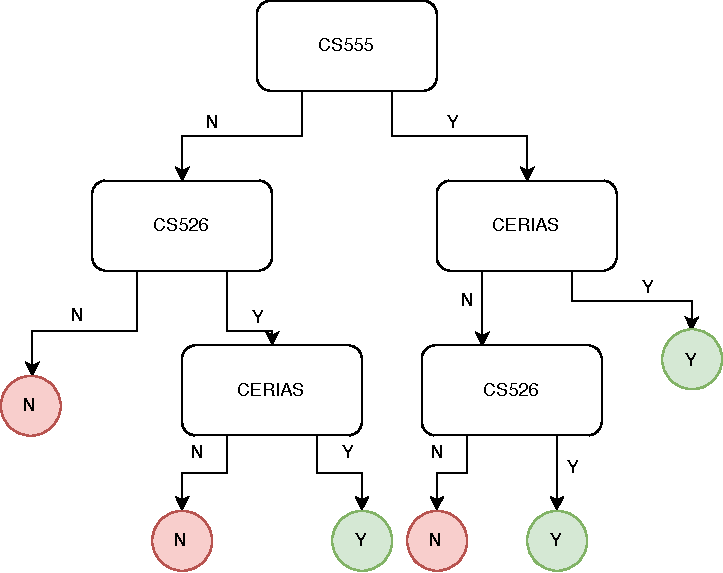
\includegraphics[scale=.75]{Information-gain.pdf}
    \caption{Decision Tree based on information gain}
    \end{figure}
    \item Gini Impurity: 
    \begin{enumerate}
        \item 
        First we need to compute the gini impurity before split:
        \begin{equation}
        \begin{split}
            Gini(\texttt{IS}) = 1 - p_y^2 - p_n^2 = 0.48
        \end{split}
        \end{equation}
        \item 
        For each of attribute, we compute:
        \begin{itemize}
             \item Cerias student: 
             \begin{equation}
             \begin{split}
             Gini(\mathsf{IS} | \mathsf{CERIAS}) &= \frac{Gini(\mathsf{IS} | \mathsf{CERIAS} = Y) + Gini(\mathsf{IS} | \mathsf{CERIAS} = N)}{2}
                                                 \\&= \frac{2 - (4/5)^2 -1/5^2 - (3/5)^2-(2/5)^2}{2} = .3999
             \end{split}
             \end{equation}
             \item CS555:
             \begin{equation}
             \begin{split}
             Gini(\mathsf{IS} | \mathsf{CS555}) &= \frac{Gini(\mathsf{IS} | \mathsf{CS555} = Y) + Gini(\mathsf{IS} | \mathsf{CS555} = N)}{2}
             \\&= \frac{2 -(5/6)^2 - (1/6)^2 - (3/4)^2-(1/4)^2}{2} = 0.3263
             \end{split}
             \end{equation}
             \item CS526:
             \begin{equation}
             \begin{split}
             Gini(\mathsf{IS} | \mathsf{CS526}) &= \frac{Gini(\mathsf{IS} | \mathsf{CS526} = Y) + Gini(\mathsf{IS} | \mathsf{CS526} = N)}{2}
             \\&= \frac{2 -(5/6)^2 - (1/6)^2 - (3/4)^2-(1/4)^2}{2} = 0.3263
             \end{split}
             \end{equation}
         \end{itemize} 
        \item Therefore, we can pick either $\mathsf{CS526}$ or $\mathsf{CS555}$ to split because it maximizes the gini difference. I chose $\mathsf{CS555}$.
         We compute entropy for left subtree and right subtree:
         \\
         On the left subtree, for each of the last 2 attributes, we compute:
         \begin{itemize}
             \item Cerias student: 
             \begin{equation}
             \begin{split}
             Gini(\mathsf{IS} |\mathsf{CS555} = N, \mathsf{CERIAS}) &= \frac{Gini(\mathsf{IS} | \mathsf{CS555} = N,\mathsf{CERIAS} = Y) + Gini(\mathsf{IS} |\mathsf{CS555} = N, \mathsf{CERIAS} = N)}{2}
             \\&= \frac{2-1/2^2 - 1/2^2 - 1-0}{2} = 0.25
             \end{split}
             \end{equation}
             \item CS526:
             \begin{equation}
             \begin{split}
             Gini(\mathsf{IS} |\mathsf{CS555} = N, \mathsf{CS526}) &= \frac{Gini(\mathsf{IS} | \mathsf{CS555} = N,\mathsf{CS526} = Y) + Gini(\mathsf{IS} |\mathsf{CS555} = N, \mathsf{CS526} = N)}{2}
             \\&= \frac{2-1/2^2 - 1/2^2 - 1-0}{2} = 0.25
             \end{split}
             \end{equation}
         \end{itemize}
         Therefore, on the left subtree, it doesn't matter which attribute is chosen.
         \\
         On the right substree, for each of the last 2 attributes,  we compute:
         \begin{itemize}
             \item Cerias student: 
             \begin{equation}
             \begin{split}
             Gini(\mathsf{IS} |\mathsf{CS555} = Y, \mathsf{CERIAS}) &= \frac{Gini(\mathsf{IS} | \mathsf{CS555} = Y,\mathsf{CERIAS} = Y) + Gini(\mathsf{IS} |\mathsf{CS555} = Y, \mathsf{CERIAS} = N)}{2}
             \\&= \frac{2-1/2^2 - 1/2^2 - 1-0}{2} = 0.25
             \end{split}
             \end{equation}
             \item CS526:
             \begin{equation}
             \begin{split}
             Gini(\mathsf{IS} |\mathsf{CS555} = Y, \mathsf{CS526}) &= \frac{Gini(\mathsf{IS} | \mathsf{CS555} = Y,\mathsf{CS526} = Y) + Gini(\mathsf{IS} |\mathsf{CS555} = Y, \mathsf{CS526} = N)}{2}
             \\&= \frac{1 - 1/3^2-(2/3)^2}{2} = 0.2222
             \end{split}
             \end{equation}
         \end{itemize}
        Therefore, on the right subtree,  we used $\mathsf{CERIAS}$ to split.
        \item Thus, this will give us the same decision as information gain. 
        \begin{figure}[h!]
        \centering
        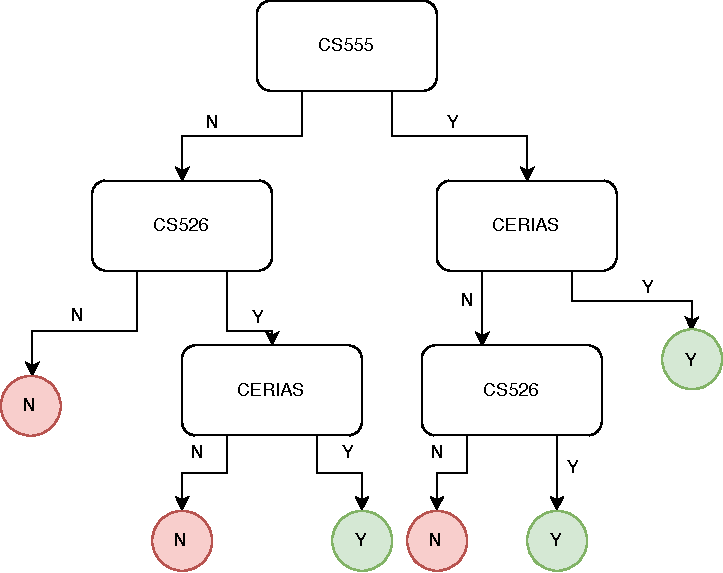
\includegraphics[scale=.75]{Information-gain.pdf}
        \caption{Decision Tree based on Gini impurity}
        \end{figure}
    \end{enumerate}
\end{enumerate}
\begin{problem}(\textbf{SVM})
Let $x_d$ denotes the number of derivation calculated,  $x_c$ denotes the number of line of codes written, \texttt{-} denotes cs student, \texttt{+} denotes math student. From the graph, we have:
\begin{table}[h!]
\centering
\begin{tabular}{c|c|c}
    $x_d$ & $x_c$ & $\mathsf{label}$\\\hline
    1 & 2 & \texttt{+}\\
    3 & 3 & \texttt{+}\\
    3 & 5 & \texttt{+}\\
    5 & 1 & \texttt{-}\\
    7 & 2 & \texttt{-}\\
\end{tabular}
\caption{Data points}
\end{table}
\begin{itemize}
    \item Compute the decision boundary. 
    \begin{proof}
        We know that the decision boundary is the line that seperate the data points into part. In otherword, it has the form of:
        \begin{equation}
            w_1x_d + w_2x_c +b =0
         \end{equation}
         and the label is determined as:
         \begin{equation}
             \mathsf{sign}(w_1x_d + w_2x_c +b)
         \end{equation}
    In other word, we need to find $(w_1,w_2,b)$ that give negative number for all math data point and positive number for all CS data points. We can simply solve the following equations:
    \begin{equation}
        \begin{split}
              &w_1 + 2w_2 + b =1
            \\&3w_1 + 3w_2 + b =1
            \\&5w_1 + 1w_2 + b =-1
        \end{split}
    \end{equation}
    we get:
    \begin{equation}
        (w_1,w_2,b) = (-1/3, 2/3, 0)
    \end{equation}
    Thus, all training data point satisfy the classifier.
    \end{proof}
    \item What is the width margin?
    \begin{proof}
        Using the equation from the class we know the width margin is:
        \begin{equation}
            \rho = \frac{2}{||w||} = \frac{2}{\sqrt{1/3^2 + (2/3)^2}} = 2.68
        \end{equation}
    \end{proof}

    \item Bob received a funny data point $(-10,5)$ from a CS student. Help Bob to build a kernel so the new SVM can classify all the data points.
    \\
    \textbf{Ans.:}\\
        \begin{table}[h!]
        \centering
            \begin{tabular}{c|c|c|c}
                $x_d$   & $x_c$ &        $\sqrt{x_d^2+x_c^2}$ & $\mathsf{label}$\\\hline
                1       & 2     &        $\sqrt{5}$ & \texttt{+}\\
                3       & 3     &        $\sqrt{18}$            & \texttt{+}\\
                3       & 5     &        $\sqrt{34}$        & \texttt{+}\\
                5       & 1     &        $\sqrt{26}$              & \texttt{-}\\
                7       & 2     &        $\sqrt{53}$       & \texttt{-}\\
                -10     & 5     &        $\sqrt{125}$              & \texttt{-}\\
            \end{tabular}
        \end{table}
        \\
        If we plot these data point into 3-d space we get:
        \begin{figure}[h!]
            \centering
            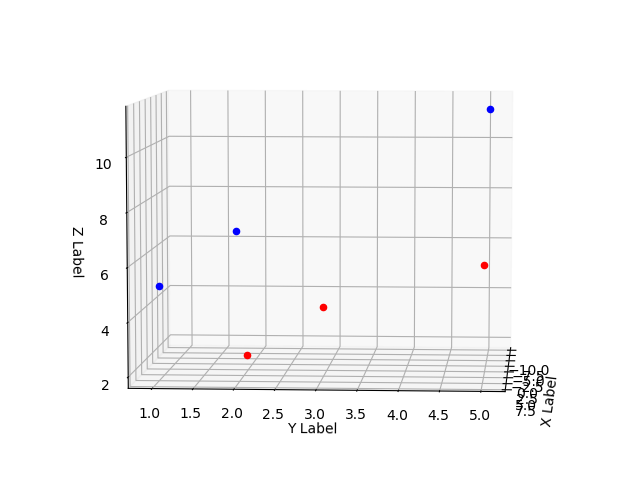
\includegraphics[scale=.5]{plot.png}
        \end{figure}
        \\
        As we can see, the data point now can be seperated by a plane. Thus, out mapping is:
        \begin{equation}
            \phi(x_d,x_c)= (x_d,x_c, \sqrt{x_d^2+x_c^2})
        \end{equation}
        The kernel is:
        \begin{equation}
        \begin{split}
            K(\mathbf{x_1},\mathbf{x_2}) &= \mathbf{x}_1\cdot \mathbf{x}_2 + ||\mathbf{x_1}||\times||\mathbf{x_2}||
                                         \\& = \phi(\mathbf{x_1}) \cdot \phi(\mathbf{x_2})
        \end{split}
        \end{equation}
        In this equation $\mathbf{x_1}\cdot \mathbf{x_2}$ denotes the dot product of 2 vectors.
    \end{itemize}
\end{problem}

\begin{problem}(\textbf{Perceptron Algorithm})
The Perceptron learning algorithm can be parameterized by a learning rate
$\alpha$. If the current weight vector $w$ classifies an instance $(\mathbf{x}, 1)$ as $-1$, we do $\mathbf{w} += \alpha \mathbf{x}$. If $(\mathbf{x}, -1)$ is
classified incorrectly as 1, we do $\mathbf{w} -= \alpha\mathbf{x}$.
\\
\textbf{3.1)} Short answers:
\begin{itemize}
    \item Assume Perceptron algorithm fails to converge on a training data D. Does adding more training data help Perceptron to converge? Justify your answer.
    \begin{proof}
        No. I think the reason is because that the algorithm is not able to find the hyperplane that seperates the current training data. Adding more training data will not help the algorithm to find the hyperplane. However, in this case, one should apply the Kernel trick or allow slack variables.
    \end{proof}
    \item What problem will result from using a learning rate that's too large, and how can one detect that problem? Justify your answer.
    \begin{proof}
        learning rate that’s too large: the decision boundary will fluctuate a lot. And so one way to detect this problem is to look at the training errors. If the training errors fluctuate without decreasing then the learning rate is too large
    \end{proof}
    \item What problem will result from using a learning rate that's too small, and how can one detect that problem? Justify your answer.
    \begin{proof}
        it will take a lot of time for perceptron to converge (assuming the data is linearly separable). 
        Also,  according to the slide, it can be very slow if two input are highly correlated.
        One way to detect this problem is to look at the training errors. if the training errors decrease very slowly then probably the learning rate is too small
    \end{proof}
\end{itemize}
\textbf{3.2)} Consider the following question about training phrase of Perceptron algorithm with training data (2
dimensional vectors) and their label.
\begin{itemize}
    \item $(0,1),0$
    \item $(1,1),1$
    \item $(1,0),1$
\end{itemize}
Assume the bias is $0$, threshold value is $0.5$, learning factor is $0.3$ and the initial weight vector is $\mathbf{w}=(0,0)$
\end{problem}
\begin{itemize}
    \item $(0,1),0:$ 
    \begin{equation*}
        \begin{split}
            (0,1) \cdot \mathbf{w} = (0,1) \cdot (0,0) = 0 \leq  0.5
        \end{split}
    \end{equation*}
    ouputs 0 which is correct.
    \item $(1,1),1:$
    \begin{equation*}
        \begin{split}
            (1,1) \cdot \mathbf{w} = (1,1) \cdot (0,0) = 0 \leq  0.5
        \end{split}
    \end{equation*}
    ouputs 0 which is not correct. We update:
    \begin{equation}
        \mathbf{w} = \mathbf{w} + \alpha \mathbf{x} =(0,0) + .3 (1,1) = (.3,.3)
    \end{equation}
    \item $(1,0),1:$
    \begin{equation*}
        \begin{split}
            (1,0) \cdot \mathbf{w} = (1,0) \cdot (.3,.3) =.3  \leq  0.5
        \end{split}
    \end{equation*}
    ouputs 0 which is not correct. We update:
    \begin{equation}
        \mathbf{w} = \mathbf{w} + \alpha \mathbf{x} =(.3,.3) + .3 (1,0) = (.6,.3)
    \end{equation}

    \item After the first 3 iteration, we have $\mathbf{w} = (.6,.3)$. We try to predict:
    \begin{equation}
    \begin{split}
        &\mathbf{x_1}\cdot \mathbf{w} = (0,0)\cdot (.6,.3) = 0 \leq .5 \text{ output } 0
        \\&\mathbf{x_2}\cdot \mathbf{w} = (1,1)\cdot (.6,.3) = 0.9 > .5 \text{ output } 1
        \\&\mathbf{x_2}\cdot \mathbf{w} = (1,0)\cdot (.6,.3) = 0.6 > .5 \text{ output } 1
    \end{split}
    \end{equation}
    Therefore, $\textbf{w}$ did accurately label all 3 samples. 
\end{itemize}
\end{document}